\chapter{Proposed Method}
\label{ch:methodology}
\label{ch:architecture}

This chapter presents RA-GARK. Section~\ref{sec:approach-principle} gives the design principle and problem setup; Sections~\ref{sec:local}--\ref{sec:cl} define the local view, KG-derived global view, rationale masking, fusion gate, and contrastive regularization; Section~\ref{sec:method-train} summarizes training and cost.

\section{Design Principle and Problem Setup}
\label{sec:approach-principle}

The failure mode identified in Chapter~\ref{ch:intro} is mandatory KG fusion. Existing KG-aware baselines inject KG embeddings into the scoring path and provide no architectural switch for ignoring KG signal when it is unreliable. RA-GARK instead follows one principle:

\begin{quote}
\emph{The KG should be a side channel whose contribution is learned by a gate, initialized toward pure collaborative filtering and opened only when the KG reduces loss.}
\end{quote}

This principle yields three design choices. First, RA-GARK has two disjoint views: a LightGCN local view $(u_{\mathrm{loc}}, i_{\mathrm{loc}})$ over the user--item graph and a KG-derived global view $(u_{\mathrm{glo}}, i_{\mathrm{glo}})$. Second, the views are combined only at the final scoring stage by user- and item-side gates. The gate bias is initialized so that $\alpha^{(0)} \approx 0.993$, making the initial model almost pure LightGCN. Third, the KG item representation is stored in $A=4$ latent aspect slots initialized by truncated SVD of an IDF-weighted item--aspect matrix and selected by softmax rationale masking.

\subsection{Architectural Overview}
\label{sec:approach-overview}

Figure~\ref{fig:architecture} shows the inference flow. The local lane applies LightGCN to obtain collaborative embeddings. The global lane looks up $u_{\mathrm{glo}}$ and forms $i_{\mathrm{glo}}$ by applying softmax weights over the item's SVD-initialized aspect slots. Fusion gates mix the two views, and the final score is an inner product. The KG-SVD step is an initialization procedure, not a forward-pass operation.

\begin{figure}[ht]
\centering

\includegraphics[width=\textwidth]{img/architecture.png}
\caption{RA-GARK architecture.}
\label{fig:architecture}
\end{figure}

\subsection{Notation}
\label{sec:approach-notation}

\begin{table}[!htbp]
\centering
\caption{Notation used in the RA-GARK formulation.}
\label{tab:notation}
\begin{tabular}{ll}
\toprule
Symbol & Meaning \\
\midrule
$\mathcal{U}, \mathcal{I}$           & sets of users and items \\
$\mathcal{R} \subseteq \mathcal{U} \times \mathcal{I}$ & observed user--item interactions \\
$\mathcal{G}_{\mathrm{KG}}$          & item--aspect knowledge graph \\
$\mathcal{A}$                        & set of aspect tags \\
$A$                                  & number of latent aspect slots per item ($A=4$) \\
$d$                                  & embedding dimension ($d=128$ unless stated otherwise) \\
$K$                                  & number of LightGCN layers ($K=2$) \\
$u_{\mathrm{loc}}, i_{\mathrm{loc}}$ & local-view embeddings \\
$u_{\mathrm{glo}}$                   & global-view user embedding \\
$\mathbf{a}_i \in \mathbb{R}^{A \times d}$ & latent aspect slots of item $i$ \\
$i_{\mathrm{glo}}$                   & global-view item embedding \\
$\alpha_u, \alpha_i$                 & user- and item-side fusion gate outputs \\
$\hat{y}(u, i)$                      & predicted preference score \\
\bottomrule
\end{tabular}
\end{table}
\FloatBarrier

\subsection{Problem Formulation}
\label{sec:approach-problem}

We study implicit-feedback top-$K$ recommendation. Given users, items, observed interactions, and an item--aspect KG, the model ranks unseen items for each user and is evaluated by NDCG, Recall, Hit Rate, and MAP.

RA-GARK scores a pair $(u,i)$ by
\begin{equation}
\label{eq:score}
\hat{y}(u, i) = \langle u_{\mathrm{final}},\ i_{\mathrm{final}} \rangle,
\end{equation}
where
\begin{equation}
\label{eq:fusion}
u_{\mathrm{final}} = \alpha_u\, u_{\mathrm{loc}} + (1 - \alpha_u)\, u_{\mathrm{glo}}, \qquad
i_{\mathrm{final}} = \alpha_i\, i_{\mathrm{loc}} + (1 - \alpha_i)\, i_{\mathrm{glo}}.
\end{equation}

Training minimizes BPR plus two auxiliary contrastive losses:
\begin{equation}
\label{eq:total-loss}
\mathcal{L} = \mathcal{L}_{\mathrm{BPR}} + \lambda_{\mathrm{CL}} \bigl( \mathcal{L}_{\mathrm{aCL}} + \mathcal{L}_{\mathrm{uCL}} \bigr),
\end{equation}
\begin{equation}
\label{eq:bpr}
\mathcal{L}_{\mathrm{BPR}} = - \log \sigma\bigl( \hat{y}(u, i^+) - \hat{y}(u, i^-) \bigr).
\end{equation}
The contrastive terms align local and global geometry with stop-gradient on the global side, and $\lambda_{\mathrm{CL}}$ is fixed at $0.005$.

\section{Local View: LightGCN}
\label{sec:local}

The local view is exactly LightGCN~\cite{he2020lightgcn}. Let $\mathbf{R}$ be the binary interaction matrix. The bipartite adjacency and normalized adjacency are
\begin{equation}
\label{eq:bipartite-A}
\mathbf{A} = \begin{bmatrix} \mathbf{0} & \mathbf{R} \\ \mathbf{R}^{\top} & \mathbf{0} \end{bmatrix},
\end{equation}
\begin{equation}
\label{eq:normalized-A}
\tilde{\mathbf{A}} = \mathbf{D}^{-1/2}\, \mathbf{A}\, \mathbf{D}^{-1/2}, \qquad \mathbf{D} = \mathrm{diag}\!\left(\mathbf{A}\,\mathbf{1}\right).
\end{equation}
Starting from trainable user and item embeddings $\mathbf{E}^{(0)}$, propagation is
\begin{equation}
\label{eq:lightgcn-prop}
\mathbf{E}^{(\ell+1)} = \tilde{\mathbf{A}}\, \mathbf{E}^{(\ell)}, \qquad \ell = 0, 1, \dots, K-1.
\end{equation}
The final local table is the layer-wise average
\begin{equation}
\label{eq:lightgcn-avg}
\bar{\mathbf{E}} = \frac{1}{K+1} \sum_{\ell=0}^{K} \mathbf{E}^{(\ell)}.
\end{equation}
We use $K=2$. No KG operation enters this branch, so $u_{\mathrm{loc}}$ and $i_{\mathrm{loc}}$ remain purely collaborative.

\section{Global View: KG-SVD Initialization}
\label{sec:kgsvd}

The global view stores item KG semantics in a learnable tensor
\begin{equation}
\label{eq:aspect-slots-def}
\mathbf{a}_i \in \mathbb{R}^{A \times d}, \qquad A = 4,
\end{equation}
collected over all items as $\mathbf{A}_{\mathrm{KG}} \in \mathbb{R}^{|\mathcal{I}| \times A \times d}$. The slots are latent directions, not raw aspect tags. They are initialized once by KG-SVD and then updated by gradient descent.

\begin{figure}[t]
\centering
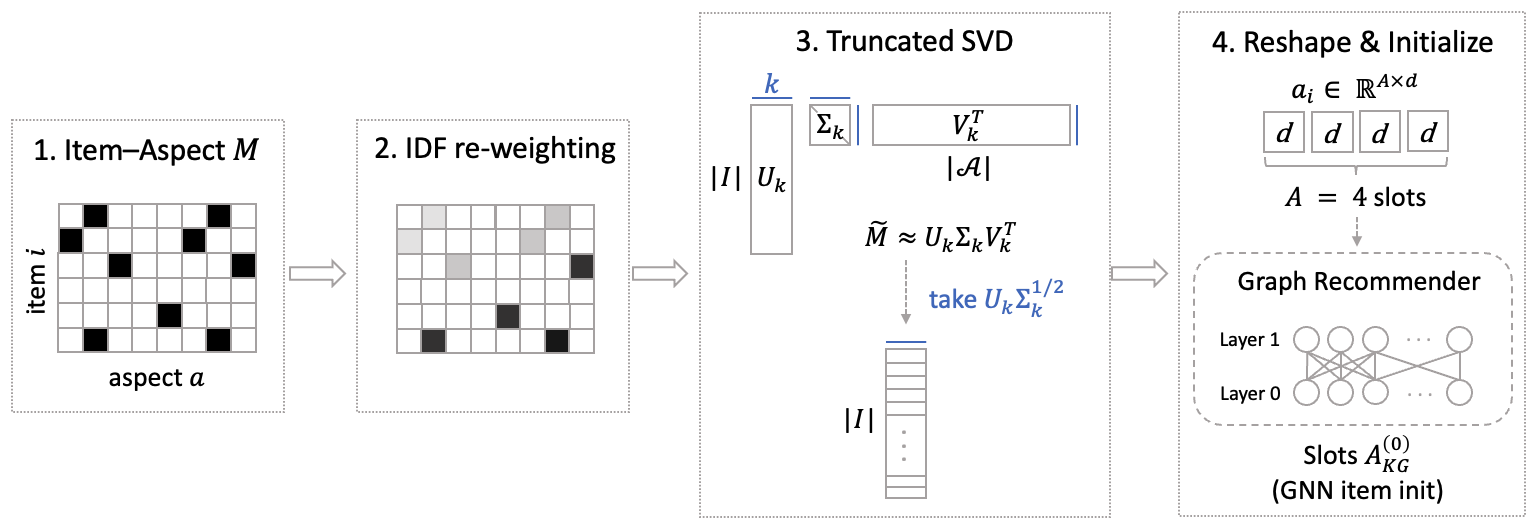
\includegraphics[width=\textwidth]{img/kg_svd.png}
\caption{KG-SVD initialization of item aspect slots.}
\label{fig:kgsvd-init}
\end{figure}

We first build the binary item--aspect matrix
\begin{equation}
\label{eq:cooc}
\mathbf{M}_{i,a} = \begin{cases} 1, & (i, a) \in \mathcal{G}_{\mathrm{KG}}, \\ 0, & \text{otherwise}. \end{cases}
\end{equation}
Frequent generic aspects are downweighted by IDF:
\begin{equation}
\label{eq:idf}
\mathrm{idf}(a) = \log\!\left( \frac{|\mathcal{I}|}{|\{i : \mathbf{M}_{i,a} = 1\}| + 1} \right) + 1,
\end{equation}
\begin{equation}
\label{eq:idf-rescale}
\tilde{\mathbf{M}}_{i,a} = \mathrm{idf}(a) \cdot \mathbf{M}_{i,a}.
\end{equation}
Then we compute the rank-$k$ SVD with $k=A d$:
\begin{equation}
\label{eq:svd}
\tilde{\mathbf{M}} \;\approx\; \mathbf{U}_k\, \boldsymbol{\Sigma}_k\, \mathbf{V}_k^{\top}, \qquad \mathbf{U}_k \in \mathbb{R}^{|\mathcal{I}| \times k},
\end{equation}
and form
\begin{equation}
\label{eq:svd-embed}
\mathbf{E}_{\mathrm{KG}} = \mathbf{U}_k\, \boldsymbol{\Sigma}_k^{1/2}.
\end{equation}
Finally, the flat item embedding is reshaped into slots:
\begin{equation}
\label{eq:reshape}
\mathbf{A}_{\mathrm{KG}}^{(0)}[i, k, :] = \mathbf{E}_{\mathrm{KG}}[i, k d : (k+1) d], \qquad k = 0, \dots, A-1.
\end{equation}
The tensor is rescaled to the Xavier-normal target standard deviation $\sqrt{2/(A+d)}$ so that KG slots start on a magnitude compatible with the other model parameters. If the aspect vocabulary were smaller than $Ad$, missing dimensions would be filled with small Gaussian noise, but this fallback is not used in our experiments.

The ablation in Section~\ref{sec:ablation-svd} shows that replacing KG-SVD with random initialization costs $6.0\%$ NDCG@20, indicating that the sparse KG does contain useful geometry but is hard to recover from random parameters.

\section{Global View: Softmax Rationale Masking}
\label{sec:softmax}

For each pair $(u,i)$, the rationale module chooses how to combine the $A$ slots of item $i$. The global user embedding is a separate lookup:
\begin{equation}
\label{eq:uglo-lookup}
u_{\mathrm{glo}} = \mathbf{E}^{\mathrm{glo}}_u, \qquad \mathbf{E}^{\mathrm{glo}} \in \mathbb{R}^{|\mathcal{U}| \times d}.
\end{equation}
For each slot $k$, the attention logit is
\begin{equation}
\label{eq:logit}
\ell_{u, i, k} = \mathrm{MLP}\!\left( [u_{\mathrm{glo}} \,\Vert\, \mathbf{a}_{i,k}] \right),
\end{equation}
with
\begin{equation}
\label{eq:mlp}
\mathrm{MLP}(\mathbf{z}) = \mathbf{w}^{\top} \cdot \mathrm{LeakyReLU}\!\left(\mathbf{W}\, \mathbf{z}\right).
\end{equation}
The same MLP is shared across slots.

The logits are normalized by a temperature-scaled softmax:
\begin{equation}
\label{eq:softmax-w}
w_{u, i, k} = \frac{\exp(\ell_{u, i, k} / \tau)}{\sum_{k' = 1}^{A} \exp(\ell_{u, i, k'} / \tau)}.
\end{equation}
We use $\tau=0.5$. The global item embedding is
\begin{equation}
\label{eq:iglo}
i_{\mathrm{glo}} = \sum_{k=1}^{A} w_{u, i, k} \cdot \mathbf{a}_{i, k}.
\end{equation}

Softmax is important because it keeps $\sum_k w_{u,i,k}=1$, bounding the scale of $i_{\mathrm{glo}}$. A sigmoid head treats slots independently and lets the embedding magnitude drift with the logits. In Section~\ref{sec:ablation-softmax}, the sigmoid variant causes the largest ablation loss. The case study later shows that the learned softmax weights are softly peaked rather than one-hot; the useful property is magnitude control for a throttled KG channel.

\section{Local-Biased Fusion and Contrastive Regularization}
\label{sec:gate}

The fusion gate implements the side-channel design. RA-GARK uses separate scalar gates for users and items:
\begin{equation}
\label{eq:gate-u}
\alpha_u = \mathrm{Gate}_{u}\!\left([u_{\mathrm{loc}} \,\Vert\, u_{\mathrm{glo}}]\right),
\end{equation}
\begin{equation}
\label{eq:gate-i}
\alpha_i = \mathrm{Gate}_{i}\!\left([i_{\mathrm{loc}} \,\Vert\, i_{\mathrm{glo}}]\right).
\end{equation}
The gates have independent parameters because the informativeness of KG signal differs by side.

\begin{figure}[ht]
\centering
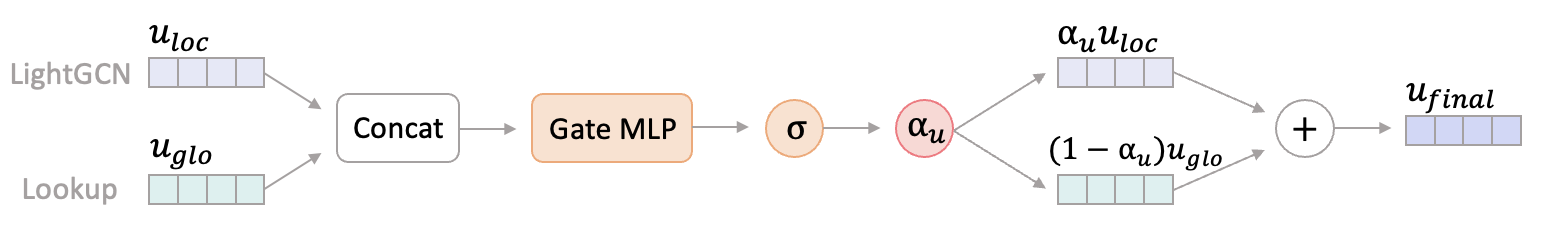
\includegraphics[width=\textwidth]{img/gate.png}
\caption{Local-biased fusion gate for combining local and global views.}
\label{fig:gate}
\end{figure}

Each gate is a small MLP with a sigmoid head:
\begin{equation}
\label{eq:gate-mlp}
\mathrm{Gate}(\mathbf{z}) = \sigma\!\left( \mathbf{w}^{\top} \tanh\!\left( \mathbf{W} \mathbf{z} \right) + b \right).
\end{equation}
The key initialization is $b=+5$, giving
\begin{equation}
\label{eq:alpha-init}
\alpha^{(0)} \approx \sigma(b) = \sigma(5) \approx 0.993.
\end{equation}
Thus the initial mixture is
\begin{equation}
\label{eq:mix-init}
u_{\mathrm{final}}^{(0)} \approx 0.993\, u_{\mathrm{loc}}^{(0)} + 0.007\, u_{\mathrm{glo}}^{(0)},
\end{equation}
and similarly on the item side. The model starts as almost pure LightGCN; gradients must push the gate open before the KG can materially affect the score. A smaller bias exposes training to KG noise, while a much larger bias makes the gate difficult to move. The sweep in Section~\ref{sec:sens-bias} supports $b=+5$.

\subsection{Cross-View Contrastive Regularization}
\label{sec:cl}

Because the two views live in different signal spaces, RA-GARK adds small contrastive losses to align their angular geometry. These losses are auxiliary; the fusion gate remains the integration mechanism.

For item slots,
\begin{equation}
\label{eq:lacl}
\mathcal{L}_{\mathrm{aCL}} = \frac{1}{A} \sum_{k=1}^{A} \mathrm{InfoNCE}\!\left( g(i_{\mathrm{loc}}),\ \mathrm{sg}\!\left[\mathbf{a}_{i,k}\right] \right),
\end{equation}
where $g$ is a projection head and $\mathrm{sg}$ is stop-gradient. InfoNCE is
\begin{equation}
\label{eq:infonce}
\mathrm{InfoNCE}(\mathbf{x}, \mathbf{y}) = -\log \frac{\exp(\langle \mathbf{x}, \mathbf{y} \rangle / \tau_{\mathrm{CL}})}{\sum_{j=1}^{B} \exp(\langle \mathbf{x}, \mathbf{y}_j \rangle / \tau_{\mathrm{CL}})},
\end{equation}
with $\tau_{\mathrm{CL}}=0.2$. The user loss is
\begin{equation}
\label{eq:lucl}
\mathcal{L}_{\mathrm{uCL}} = \mathrm{InfoNCE}\!\left( g(u_{\mathrm{loc}}),\ \mathrm{sg}\!\left[u_{\mathrm{glo}}\right] \right).
\end{equation}
Stop-gradient prevents the contrastive objective from overwriting the SVD-initialized KG geometry; the local view absorbs the alignment cost.

\section{Training and Computational Complexity}
\label{sec:method-train}

\subsection{Total Objective}
\label{sec:train-objective}

The full objective is \Eqref{eq:total-loss}: BPR provides the ranking signal, and the two contrastive terms provide weak cross-view alignment.

\subsection{Optimization}
\label{sec:train-opt}

We train with Adam, learning rate $10^{-3}$, batch size $128$, for up to $80$ epochs. Early stopping uses validation NDCG@20 with patience $10$. Each batch contains triplets $(u,i^+,i^-)$, with $i^-$ sampled uniformly from unobserved items for user $u$.

\subsection{Inference}
\label{sec:train-inference}

At inference time, LightGCN propagation is computed once and cached. For each user, item scores are computed in a vectorized pass over all candidate items, including rationale masking, item gating, and the final inner product.

\subsection{Computational Complexity}
\label{sec:train-complexity}

\begin{table}[!htbp]
\centering
\caption{Per-batch training cost of RA-GARK modules.}
\label{tab:complexity}
\begin{tabular}{ll}
\toprule
Module & Cost \\
\midrule
LightGCN propagation       & $O(|\mathcal{E}_{\mathcal{U}\mathcal{I}}|\, d\, K)$ \\
$u_{\mathrm{glo}}$ lookup  & $O(B\, d)$ \\
Aspect-slot read           & $O(B\, A\, d)$ \\
Rationale masking          & $O(B\, A\, d)$ \\
User and item fusion gates & $O(B\, d^2)$ \\
BPR + contrastive losses   & $O(B\, d)$ \\
\bottomrule
\end{tabular}
\end{table}
\FloatBarrier

The dominant term is LightGCN propagation, as in the baseline. The KG additions are linear in $A$ and $d$ except for the small gate MLPs, and remain a small constant-factor overhead at $A=4$.
